\documentclass{techbrief}

\title{Data\! Visualization}
\date{\today}
\event{Special Report}

\newcommand{\modulus}{\textsf{Modulus}}

\usepackage{lipsum}

\begin{document}
\newgeometry{margin=1cm,headheight=3cm,includehead,includefoot}
\pagestyle{main}%\onecolumn
\thispagestyle{title}
\pagenumbering{gobble}
\lettrine[lines=2]{A}{} promised feature of \modulus\ is rich data
visualization---even when in
aggregate.
In this document we will describe issues and needs of instructors of `Big-Math
5000,' a fictitious course of 5000 students.
Issues that are relevant to \modulus\ include:
\begin{enumerate}
    \item There are many `roles' that instructors have: Course Coordinator,
          Lecturer, Teaching Assistant. How do we push this work back to
          Big-Math 5000?
    \item What sort of meaningful aggregate data can we give?
    \item How can we display this data in a meaningful way?
\end{enumerate}

We believe \modulus, despite its minimal interface, will be capable of dealing
with issues.

\begin{xframe}{\bfseries \modulus} is our assignment database. It will provide
    (among other things) LTI connection to Canvas.

    \begin{center}
        \begin{tikzpicture}
            \node at (-3,1) [cloud, draw,cloud puffs=10,cloud puff arc=120,
                aspect=2, inner ysep=1em,scale=.8] {};
            \node at (-3,1) {LMS};
            \node at (-3,-1) {\resizebox{1cm}{!}{\documentclass[tikz]{standalone}
\begin{document}
\begin{tikzpicture}[rounded corners=.1pt]
    \draw (-.15,-.1) rectangle (.95,.5);
    \draw[fill=white] (0,0) rectangle (1,.8);
    \draw[fill=white] (0,0) -- (-.2,.1) -- (-.2,.9) -- (.8,.9) -- (1,.8) -- (0,.8) --
    cycle;
    \draw (0,.8) -- (-.2,.9);
    \draw[fill=white] (0,-.05) -- (1,-.05) -- (1,-.25) -- (0,-.25) -- cycle;
    \draw[fill=white] (0,-.05) -- (0,-.25) -- (-.2,-.15) -- (-.2,.05) -- cycle;
    \draw[rounded corners=.5pt,fill=gray] (.1,.1) rectangle  (.9,.7);
    \draw (-.2,-.25) -- (1.1,-.25) -- (1.2,-.37) -- (-.1,-.37) -- cycle;
    \draw (-.2,-.25) -- (-.2,-.3) -- (-.1,-.4) -- (-.1,-.37) -- cycle;
    \draw (-.1,-.4) rectangle (1.2,-.37);
\end{tikzpicture}
\end{document}}};
            \node at (-3,-2) {Students with LTI};
            \draw[->] (-3.1,-.4) -- (-3.1,.4);
            \draw[<-] (-2.9,-.4) -- (-2.9,.4);
            \node at (0,0) {\resizebox{1cm}{!}{\documentclass[tikz]{standalone}
\begin{document}
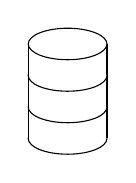
\begin{tikzpicture}[rounded corners=.5pt]
    \draw[fill=white] (.5,0) ellipse (.5cm and .2cm);  


    \draw[draw=none,fill=white] (0,0) rectangle (1,.4);
    \draw[] (0,0) -- (0,.4);
    \draw[] (1,0) -- (1,.4);    
    \draw[fill=white] (.5,.4) ellipse (.5cm and .2cm);  

    \draw[draw=none,fill=white] (0,.4) rectangle (1,.8);
    \draw[] (0,.4) -- (0,.8);
    \draw[] (1,.4) -- (1,.8);    
    \draw[fill=white] (.5,.8) ellipse (.5cm and .2cm);  


    \draw[draw=none,fill=white] (0,.8) rectangle (1,1.2);
    \draw[] (0,.8) -- (0,1.2);
    \draw[] (1,.8) -- (1,1.2);    
    \draw[fill=white] (.5,1.2) ellipse (.5cm and .2cm);  
\end{tikzpicture}
\end{document}}};
            \node at (0,-1) {\modulus};
            \draw[->] (-2,.8) -- (-.6,.2);
            \draw[<-] (-2.1,.6) -- (-.7,0);
            \node at (3,-1) {\resizebox{1cm}{!}{\documentclass[tikz]{standalone}
\begin{document}
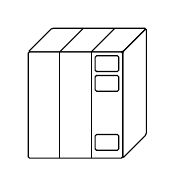
\begin{tikzpicture}[rounded corners=.5pt]
    \draw (0,0) rectangle (1.2,1.35);
    \draw (.4,0) -- (.4,1.35);
    \draw (.8,0) -- (.8,1.35);

    \draw (0,0)+(.85,1.1) rectangle ([shift={(.85, 1.1)}] .3, .2);
    \draw (0,0)+(.85,.85) rectangle ([shift={(.85, .85)}] .3, .2);
    \draw (0,0)+(.85,.1) rectangle ([shift={(.85, .1)}] .3, .2);

    \draw (1.2,0) -- (1.2,1.35) -- (1.5,1.65) -- (1.5,.3) -- cycle;

    \draw (0,1.35) -- (.3,1.65) -- (1.5,1.65) -- (1.2,1.35) -- cycle;
    \draw (.4,1.35) -- (.7,1.65);
    \draw (.8,1.35) -- (1.1,1.65);    
\end{tikzpicture}
\end{document}}};
            \node at (3,-2) {Ximera};
            \node at (3,-2.4) {Server};
            %\node at (3,1) {\resizebox{1cm}{!}{\documentclass[tikz]{standalone}
\begin{document}

\begin{tikzpicture}[rounded corners=.1pt]
    \draw (-.15,-.1) rectangle (.95,.5);
    \draw[fill=white] (0,0) rectangle (1,.8);
    \draw[fill=white] (0,0) -- (-.2,.1) -- (-.2,.9) -- (.8,.9) -- (1,.8) -- (0,.8) --
    cycle;
    \draw (0,.8) -- (-.2,.9);
    \draw[fill=white] (0,-.05) -- (1,-.05) -- (1,-.25) -- (0,-.25) -- cycle;
    \draw[fill=white] (0,-.05) -- (0,-.25) -- (-.2,-.15) -- (-.2,.05) -- cycle;
    \draw[rounded corners=.5pt,fill=gray] (.1,.1) rectangle  (.9,.7);
    \draw (-.2,-.25) -- (1.1,-.25) -- (1.2,-.37) -- (-.1,-.37) -- cycle;
    \draw (-.2,-.25) -- (-.2,-.3) -- (-.1,-.4) -- (-.1,-.37) -- cycle;
    \draw (-.1,-.4) rectangle (1.2,-.37);
\end{tikzpicture}
\end{document}}};
            %\node at (3,2) {Self-learner};
            % \draw[->] (3.1,-.4) -- (3.1,.4);
            % \draw[<-] (2.9,-.4) -- (2.9,.4);
            %\draw[->] (2,.8) -- (.6,.2);
            %\draw[<-] (2.1,.6) -- (.7,0);
            \draw[->] (2.3,-1) -- (.6,-.4);
            \draw[<-] (2.4,-.8) -- (.7,-.2);
        \end{tikzpicture}
    \end{center}
    For students using a supported LMS, modulus

    Its basic functionality is that it will provide a course ID. In this case
    the course ID for Big-Math 5000 is \texttt{12345}. This should probably be
    a
    random hash.
    Any URL appended to
    \begin{center}
        \texttt{https://modulus.org/12345/}
    \end{center}
    number of submissions.
    will \textit{automatically} become part of the Big-Math 5000 data set.
\end{xframe}

\break

\begin{xframe}
    \textbf{Big-Math 5000} is a coordinated course. This means there are
    \textit{Course Coordinators} who oversee the entire course of 5000
    students,
    there are \textit{Lecturers} who have classes of 200, and there are
    \textit{Teaching
        Assistants} who teach sections of 40.

    Course Coordinators need to be able to `Set-up' a course in
    \textsl{Canvas}, and then copy
    this course for their 25 lecturers. They use the same 100 assignments each
    semester. Identical copies of the course (from the view of the LMS) must
    function.  There are 2 additional assignments in this
    course, 1 unique to each lecturer, and 1 unique to each recitation
    instructor. No mass-editing can be done. Hence they want a single
    identifier for Big-Math 5000,
    \begin{center}\scriptsize
        \texttt{https://modulus.org/12345/https://assignment001}\\
        \texttt{https://modulus.org/12345/https://assignment002}\\
        \texttt{https://modulus.org/12345/https://assignment003}\\
        \dots\\
        \texttt{https://modulus.org/12345/https://assignment100}\\
    \end{center}
    This identifier will \textbf{not change} between sections of Big-Math 5000,
    nor will it change between semesters or years. If someone has rights to see
    data in \modulus\ for Big-Math 5000, they will be able to see the data for
    the history of the course.

    Moreover, Course Coordinators need to be able to see data for all students
    \textbf{scaled} and \textbf{grouped} by \textbf{lecture} and
    \textbf{recitation}.

    As a \textbf{solution} to these issues, instructors will have a
    personalized
    \modulus\ assignment that they give all of their courses. If Jim Fowler and
    Bart Snapp are Teaching Assistants in Big-Math 5000, then they each give
    their
    students the respective assignments:
    \begin{center}\scriptsize

        \texttt{https://modulus.org/12345/https://ximera.osu.edu/meetJimFowler}\\

        \texttt{https://modulus.org/12345/https://ximera.osu.edu/meetBartSnapp}\\
        \dots
    \end{center}
    And now the Course Coordinator knows which student is in which section
    simply by the assignments the student submitted.
\end{xframe}

\begin{xframe}
    \textbf{The data} for a given assignment that we seek are
    \begin{description}
        \item[Percent complete] This is essentially the grade on the assignment
        \item[Completion over time] This is how the completion of the activity
            it takes to complete an activity. Fit sigmoids to the student time series data.
            % \item[Attempts to Completion] This would be the total number of answers
            %     submitted necessary to complete the activity; perhaps divided by
            %     the (total!) number of answerables.
            % \item[First Attempt] Percent complete on first
            %     attempt. All assignments are valued
            %     0--1. If an assignment has 4 questions and a student gets
            %     all 4 correct on the first attempt, then this would be 100\%. If
            %     the student gets the first question correct on the first attempt,
            %     and every other question takes more attempts, then this is 25\%.
    \end{description}
\end{xframe}

\begin{xframe}
    \textbf{\modulus} should provide something equivalent or better than the
    what follows. The(/an?) owner of 12345 should be able:
    \begin{description}
        \item[List] all 12345 assignments filtered by a \textbf{minimum number
                of unique student attempts/completions} (which could be 0) in a
            given \textbf{date-range}.
        \item[Select] data from a \textbf{assignment-list} that is pasted into
            \modulus\ along with a \textbf{date-range}. This list of
            assignments could be
            generated in the step above.
        \item[View] the \textbf{data} for the \textbf{assignments selected
                above},
            for \textbf{students} who \textbf{attempted/completed any/all}
            assignments in a
            \textbf{list}, usually part of the list in the first step.
            filtered by a \textbf{minimum number
                of unique student attempts/completions} (which could be 0) and
            a
            \textbf{date-range}.
    \end{description}
\end{xframe}

\begin{xframe}
    \textbf{Visualizing} this data will be achieved via a heat map in an
    student-assignment matrix:
    \begin{center}
        \begin{tikzpicture}
            \node[anchor=north west] at (-.2,.5) {\scriptsize 100 common
                assignments};
            \node[anchor=north west] at (-.5,-.4) {\rotatebox{90}{\scriptsize
                    200
                    anonomous students along the side}};
            \node[anchor=north west] at (0,0)
            {
\includegraphics[width=3cm]{lecture.png}};
            \node[] at (5,-2) {\scriptsize Unique};
            \node[] at (5,-2.3) {\scriptsize recitation assignments};

            \draw[->] (3.8,-2.3) -- (3.2,-.5);
            \draw[->] (3.8,-2.3) -- (3.2,-1.5);
            \draw[->] (3.8,-2.3) -- (3.2,-2.3);
            \draw[->] (3.8,-2.3) -- (3.2,-3.3);
            \draw[->] (3.8,-2.3) -- (3.2,-4.3);

            \draw[->] (4,-5.2) -- (2.5,-4.7);
            \node[] at (4,-5.5) {\scriptsize Unique lecture  assignment};

        \end{tikzpicture}
    \end{center}
    Here, darker colors might corresponds to ``fewer attempts to completion,''
    ``less time to completion,'' or ``fewer correct on first attempt.''
    However,
    the ideal coloring can be left for another time.

    With such a visualization, we would be able to better understand the
    difficulty of our assignments, and see if differences in performance occur
    between recitations/lectures.
\end{xframe}

\begin{xframe}
    \textbf{Further analysis} of the data should be available via
    collapsing and zooming.

    \textit{Collapsing} the data means taking some average of student work, to
    simply
    analyze the assignments and taking averages of assignments to analyze
    student
    performance. Once data is collapsed, there are other, more common (bar
    chart,
    scatter plot, line graph etc) that can be used.

    \textit{Zooming} the data means making the heat map larger.
    As an example, perhaps if we zoom-in and hover, we find:
    \begin{center}
        \begin{tikzpicture}
            \node at (0,0) {
\includegraphics[width=7cm]{zoom.png}};
            \node[fill=white,notice={(-1,-.8)}, text width=3.5cm] at (-.7,.5)
            {\begin{minipage}{3.5cm}\scriptsize\ttfamily
                    https://assignment054\\ 85
                    percent to completion
                \end{minipage}};
        \end{tikzpicture}
    \end{center}
    Clicking on the individual assignments could show a heat map of student
    activity.
\end{xframe}

\begin{xframe}
    \textbf{Accessibility} is difficult with this setting; however, we could
    provide export to a basic 3D printing of this diagram.
\end{xframe}

\restoregeometry
\onecolumn\noindent
With this model of visualization, flexible \textbf{sorting options}, ways to
\textbf{discard erroneous assignments}, and \textbf{options for the range of
    the heat map}, we should be able to effectively visualize the entire
course,
with a mock-up given below:
\begin{center}

    
\includegraphics[width=3cm]{course1-5.png}
\includegraphics[width=3cm]{course6-10.png}
\includegraphics[width=3cm]{course11-15.png}
\includegraphics[width=3cm]{course16-20.png}
\includegraphics[width=3cm]{course21-25.png}
\end{center}
Here we see the data for all assignments for the entire 5000 student course.
With this set-up, we would be able to identify problematic assignments and
issues in the course.

% \begin{xframe}
%     \textbf{Funding for the Ximera Project} is provided by
%     a U.S.\ Department of Education Open Textbooks Pilot Program grant in the
%     amount of \$2,125,000, from 2024--2026, with no external funding. In the
%     past, the Ximera Project has
%     also received support from NSF Grant DUE-1245433, the Shuttleworth
%     Foundation, the Ohio State University
%     Department of Mathematics, and the Affordable Learning Exchange at OSU.
% \end{xframe}

\end{document}